\documentclass[main.tex]{subfiles}

\begin{document}

\section{Matching Algorithms}
The matching problem is solved on the static graph every $n_{match}$ steps. One goal for the optimization algorithms is to find the maximum edge-disjoint cycle covering, which can be solved as Min-D-DCC is solved \cite{Man1} \cite{Bir}. The section \ref{bima} discusses this PTIME algorithm. This is optimal for $p=1$.

With $p<1$, the matching problem is to find the maximum cycle-weight edge-disjoint cycle covering, where cycle weight is $\E[c_k] = k p^k$. This problem is NP-Hard and APX-Complete \cite{Bir}. See Dickerson \cite{Dick} \cite{Dick3} for the state-of-the-art ILP (integer linear programming) solving this problem for kidney exchange.

An alternate approximation is to find the maximum edge-disjoint covering with cycles of length $\leq k$. The complexity is, however, identical. Bir\'{o} \cite{Bir} provide an exact graph algorithm to solve this. There are many good ILP techniques providing exact solutions as well. See \cite{And3} \cite{Glo1} \cite{Pla} \cite{Dick1}. ILP algorithms are easier to add new features to.

\subsection{Maximum Edge-Weight Matching (MAX-WEIGHT)}\label{bima}

The standard algorithm to find a maximum edge-weight edge-disjoint cycle covering in PTIME transforms the graph into a bipartite graph and then finds a perfect weighted matching \cite{Bir}. The

The bipartite graph has one side for Offers and one for Requests. For each ORpair, (offer=$task_a$, request=$task_b$), create two nodes with edge weight $0$. Next an edge is created between the offer node and every request node for $task_a$ with weight $> 0$. Then a maximum weight perfect matching algorithm can be used. A positive weighted edge for an offer can only be matched if the corresponding request has a positive weighted edge match; if the ORpair is in no cycle, then the $0$ weight edge is mached.

The bipartite graph has $2*|ORpairs|$ nodes and $\bO(|ORpairs|^2)$ edges. The perfect weighted matching can be found via Munrkes algorithm or the Hungarian algorithm in $\bO(n^3)$ time.

The positive weight can be used to assign preferences to some ORpairs over others, perhaps due to user preferences (soft constraints), proportional to task popularity (degree), or according to reputation. Weights could also be used to represent non-uniform acceptance probability, which may be a useful heuristic.

The drawback of this algorithm is that long-cycles are possible, and in a dense graph, such as for kidney exchange, very likely.

\subsection{Maximum 2-way Matching (MAX-2)}
In the case that $p < 0.7$, a simple 2-cycle cover will likely perform best. Also $\bO(n^3)$.

This can be followed up by another algorithm, such as MAX-WEIGHT.

\subsection{Greedy Shortest Cycle (GSC)}\label{sec:gsc}
A simple heuristic is to pick an arbitrary node, find the shortest cycle\footnote{For example, using Dijkstra's algorithm}, and then mark the nodes as matched. Repeat this process until there are no more cycles in unmatched nodes.

The rationale is that for $p < 0.85$ cycles of length $k < 10$ are optimal, and specifying an exact cycle length cap may not provide much additional gain.

The run-time is $\bO((|ORpairs| + |tasks|\ln|tasks|)|ORpairs)$; however, many the search for many ORpairs will be cut short because of already matched cycles.

\subsubsection{Relation to Maximal and Greedy (GSC-M)}
GSC is similar to Maximal and Greedy in Abbassi \cite{Abb1}. However, Maximal chooses any cycle and Greedy finds the maximum weight cycle, which is slow. As with Maximal, running GSC $M$ times and choosing the best cover may result in significantly better results.

\subsubsection{Product of Degrees Order (GSC-POD)}
Jia \cite{Jia1} find that ordering the nodes prior to running a greedy shortest cycle cover algorithm boosts results. This seems wise with GSC as well. The reasoning is that a cycle for an ORpair with a well-connected, popular, task may use up the only cycle for an unpopular task. An additional perk of finding the shortest cycle is that this cycle is less likely to use up an ORpair needed by another ORpair unpopular task.

\subsection{Dynamic Shortest Cycle (DYN-SC)}
Dynamically find shortest cycles involving just added ORpairs every few (1 to 10) steps.

DYN-SC is very similar to GSC. DYN-SC is faster but may miss cycles involving matched ORpairs that did not accept their matches, unless these are also included.

\subsection{Hanging ORpairs (HOR)}
\begin{figure}
  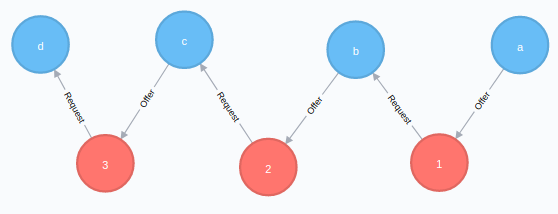
\includegraphics[width=\textwidth]{hanging_example.png}
  \caption{1,2,3 are ORpairs and a,b,c,d are task nodes.}
  \label{hanging_example}
\end{figure}

In the mid-p, $0.7 < p < 0.95$, range, long cycles will be rejected with high probability. This MAX-WEIGHT infeasible. The Hanging ORpair approach seems to salvage a long cycle with only a few rejectors.

The Hanging ORpair approach is best exemplified by the following two acceptance scenarios for the case in Figure \ref{hanging_example} where ORpairs $1$, $2$ and $3$ are part of a larger cycle:
\begin{itemize}
  \item Users $1$, $2$, and $3$ accept the match: consider ORpair $2$ satisfied. User $2$ gives $task_b$ to user $1$ and gets $task_c$ from user $3$.
  \item Users $1$ and $3$ accept, but user $2$ rejects the match: consider an ORpair like $2$ as all that's needed to fix the match. Create a new, hanging, ORpair for users $1$ and $3$: (offer: $task_c$, request: $task_b$), the converse of ORpair $2$.
\end{itemize}

The core idea is that a match being found implies parity among the tasks involved ($a, b, c, d, \dots$). Thus odds are there will be more matches for the new ORpair. Gambling on this, long cycles and 3-cycle coverings can expect the same number of satisfied ORpairs.

Algorithmically speaking, MAX-WEIGHT can be used in the mid-p rangeto find the maximum weight edge-disjoint cycle cover, and rejectors and hanging ORpairs can be rematched. This is preferable to other methods because there will still be as many rejectors (as $p$ is uniform).

Finally, when multiple adjacent users in a match reject, the acceptors on either side of the streak can be joined to form a hanging ORpair.

\subsubsection{Theoretical Drawbacks}\label{sec:theoretical drawbacks}
Some theoretical drawbacks concern the fact that the parity assumption is not always generalizable.

\begin{itemize}
  \item Subjective value of tasks and willingness to trade for other tasks varies. A hanging ORpair replacing an ORpair of a user with unusual subjective value of a task may be harder to rematch. The example given in Cabinallas \cite{Cab0} of Kyle MacDonald trading a paper clip for a house demonstrates this effect.
  \item A task in the hanging ORpair could also be very rare or unpopular, resulting in a long wait time.
  \item A task could have lower acceptance probability.
\end{itemize}

These situations could result in one user being markedly worse off in the HOR approach. And if not, they could worsen the practical drawbacks.

A user's ORpair is not expected to be held more than 1-2 times in the mid-p range (see section \ref{sec:nrounds}), but this says nothing about the wait time between rounds.

Additional drawbacks:
\begin{itemize}
  \item The acceptance probability for the Hanging ORpair is also likely to change as now two users need to accept whatever match it's in.
  \item ORpair expiration or tasks that need to be done in good time cannot be handled easily.
  \item An ORpair whose offer and request need to be done at the same time cannot be held.
\end{itemize}


\subsubsection{Practical Drawbacks}
Ideally, a sure will upload an ORpair to the offer network, get a match notification, evaluate the option. If the user accepts the match, the user will work on vis offer and wait for vis request. If the user rejects, the user simply waits for another match.

HOR complicates the user experience to facilitate better global performance, and as noted in \ref{sec:theoretical drawbacks}, HOR risks elongating a user's wait time.

In Figure \ref{hanging_example},
\begin{itemize}
  \item User $3$ is asked to receive $task_d$ and keep offering $task_c$ for an indefinite period.
  \item User $1$ is asked to give $task_a$ and wait for $task_b$ for an indefinite period\footnote{Interestingly, if the offer network is used by computer agents performing speculative execution, this problem diminishes as user $1$ may compute $task_a$ prior to knowing whether the match is accepted or not.}.
\end{itemize}

First, this complications may make HOR an opt-in feature as there are risks the user has to accept. HOR won't work if there aren't enough users opting in. Practically, users may also have to accept each particular case of creating a new hanging ORpair, to, e.g., prevent a high reputaiton and low reputation user from being joined together: this will make the communication protocol and user experience more complicated, as well as increase the time to determine the acceptance of a match.

Next: what incentive is there for user $3$ to keep offering $task_c$ instead of just quitting after receiving request $task_d$? In the kidney case, encouraging anyone to donate a kidney is immoral (and illegal), so exchanges \textit{must} be simultaneous, and chains are started by a donation, so reneging is permissible. In general, a contract is needed: by accepting $task_d$ user $3$ accepts to do $task_c$ or else be penalised.

A standard way to do this is via a reputation system\footnote{\url{https://en.wikipedia.org/wiki/Reputation_system}}. In a reputation system users are given a reputation score, usually based on user feedback. For example, on eBay, feedback describes whether the seller shipped on time and provided the item as described. The reputation score is calculated from the total feedback of the sellar. Users strongly avoid buying from a seller with negative feedback \cite{ebay}. Sellers with high reputation on eBay can sell the same item at a higher price, or on Taobao\footnote{A Chinese site like eBay.}, which has a thicker market, sell more of an item \cite{Ye1}.

In an offer network, users could get feedback on tasks they offer after accepting a match. A user accepting a match and then not delivering will result in negative feedback. Users will be very likely to reject a match with a user with negative feedback\footnote{Reputation can also be part of the matching system; although this makes the entry barrier harder for new users.}. In this way, the reputation system largely prevents users from leaving after they receive their request.

\subsubsection{Offer Reneging}
The above discussion is about an algorithm users can opt in to \textit{prior} to binding acceptance of a match. Users well, however, accept a match and then renege and not deliver the offered task. A reputation system can make it hard for the user to find new matches in the future, but the user promised vis request needs to be dealt with as well. A hanging ORpair cannot be created with just one hanging request.

Without gifts or asynchronicity\footnote{Asynchronous exchange is mentioned by Abbassi \cite{Abb2}, but only implemented via a credit system.}, the only option is to, unfortunately, ask the user to re-upload his ORpair with a higher weight next time the matching system is run. Or, perhaps, to immediately  This would result in the user giving an offer twice; otherwise, the same reneging problem would propogate around the cycle.

A queue, like the cadaver queue in kidney exchange, provides additional options. The user can opt to place vis offer in a reasonable position in the queue. One way for the request queue to be satisfied is via (altruistic) users givig the task for free (as kidney donors do). Another is to allow users to upload asynchronous ORpairs: that is, a user is willing to do the offer for a user in the request queue in exchange for the user's place\footnote{This is similar to the \textit{you request
my house—I get your turn} variant of Top Trading Cycles proposed by Abdulkadiro{\u{g}}lu, Atila and S{\"o}nmez \cite{abd1}}. A chain starting with a gift and ending in the request queue is then also an option. A user could also be willing to accept vis request as a gift prior to vis offer being matched.

\subsubsection{HOR and Asynchronous Exchange}
An alternative to creating a new hanging ORpair is to add the request to the queue and treat the offer as a gift. From this perspective, HOR is, in essence, looking for chains from a specific giver to a specific requester.

A method of finding chains that avoids special processing is to create a dummy task that all lone requests offer and all lone offers request. This would allow for a generalization of HOR where any held offers or requests can be matched up together. This method, however, does not work well with altruistic gifts.

\end{document}

%%Used to generate Hanging ORpair figure:
% CREATE (t1:Task {id:'a'})
% CREATE (t2:Task {id:'b'})
% CREATE (t3:Task {id:'c'})
% CREATE (t4:Task {id:'d'})
% CREATE (o1:ORpair {id:'1', offer:'a', request:'b', user:'1'})
% CREATE (o2:ORpair {id:'2', offer:'b', request:'c', user:'2'})
% CREATE (o3:ORpair {id:'3', offer:'c', request:'d', user:'3'})
% CREATE (t1)-[:Offer]->(o1)-[:Request]->(t2)
% CREATE (t2)-[:Offer]->(o2)-[:Request]->(t3)
% CREATE (t3)-[:Offer]->(o3)-[:Request]->(t4)


% \subsection{Matching via Weighted Boolean Optimization}
% Note: this section should perhaps be deleted in favor of simply a description of the work Abraham et al. \cite{Abr1} have done.
%
% One linear programming formulation of the problem is for weighted boolean optimization \cite{Mar1}.
%
% The variables:
% \begin{itemize}
  % \item Let $x_{abt}$ denote $u_a$ doing $t_t$ for $u_b$
  % \item Let $r_{at}$ denote a task $u_a$ requests for offered task $t_t$.
%
        % That is, an edge: $(t_t, r_{at})$ : $u_a$
  % \item Let $s_{at}$ be a selection varable indicating whether $u_a$'s request $t_t$ is satisfied
  % \item Let $w_{abt}$ be a weight describing $u_a$'s satisfaction with $u_b$ fulfilling request $t_t$
% \end{itemize}
%
% Denote $U$ the set of users and $T$ the set of tasks
% The constraints for each user $a \in U$ and $t \in T$:
% \begin{enumerate}
  % \item $\sum_{b \in U} x_{abt} \leq 1$
  % \item $sum_{b \in U} x_{abt} = \sum{b \in U} x_{bar_{at}}$
  % \item $s_{at} + \sum_{b \in U} x_{bar_{at}} > 1$
% \end{enumerate}
%
% Minimize:
  % $$\sum_{a \in U, b \in U, t \in T} w_{abt} s_{at}$$
%
% One the positive side, a lot of work has gone into good linear program and SAT solvers despite the problem being NP-complete. Furthermore, additional features are easy to add into the formulation.
%
